\documentclass[a4paper, 11pt]{article}
% Esto es para poder escribir acentos directamente:
\usepackage[latin1]{inputenc}
% Esto es para que el Latex sepa que el texto está en español:
\usepackage[spanish]{babel}

\usepackage[latin1]{inputenc}

%Paquetes de la AMS:
\usepackage{amsmath, amsthm, amsfonts}

\usepackage{enumitem}
\usepackage{float}
\usepackage{graphicx, epstopdf}
\usepackage{epsfig}
\usepackage{wrapfig}
\usepackage{svg}

\newtheorem{Teo}{Teorema}[section]
\newtheorem{Cor}{Corolario}
\newtheorem{Lem}{Lema}
\newtheorem{Prop}{Proposición}
\newtheorem{Def}{Definición}
\theoremstyle{definition} \theoremstyle{remark}
\newtheorem{Obs}{Observación}

\title{Tarea 3 Redes de Telecomunicaciones}
\author{Gonzalo Olvera Monroy}

\begin{document}
    \maketitle
    \section{R4. Describa por qu\'e un desarrollador de aplicaciones podr\'ia elegir ejecutar una aplicaci\'on sobre UDP en lugar de TCP.}
    Un desarrollador de aplicaciones puede no querer que su aplicaci\'on utilice el control de congesti\'on de TCP, que puede reducir la tasa de env\'io de la aplicaci\'on en momentos de congesti\'on. A menudo, los dise\~{n}adores de aplicaciones de telefon\'ia IP y videoconferencia IP eligen ejecutar sus aplicaciones sobre UDP porque quieren evitar el control de congesti\'on de TCP. Adem\'as, algunas aplicaciones no necesitan la transferencia de datos confiable proporcionada por TCP.

    \section{R5. ?`Por qu\'e es que el tr\'afico de voz y v\'ideo a menudo se env\'ia a trav\'es de TCP en lugar de UDP en la Internet de hoy? (Sugerencia: La respuesta que estamos buscando no tiene nada que ver con el mecanismo de control de congesti\'on de TCP.)}
    Dado que la mayor\'ia de los firewalls est\'an configurados para bloquear el tr\'afico UDP, el uso de TCP para el tr\'afico de video y voz permite que el tr\'afico atraviese los firewalls.

    \section{R6. ?`Es posible que una aplicaci\'on disfrute de una transferencia de datos fiable incluso cuando la aplicaci\'on se ejecuta sobre UDP? Si es as\'i, ?`c\'omo?}
    Si. El desarrollador de la aplicaci\'on puede transferir datos confiables al protocolo de la capa de la aplicaci\'on. Sin embargo, esto requerir\'ia una cantidad significativa de trabajo y depuraci\'on.

    \section{R12. Visite el applet Go-Back-N Java en el sitio Web adjunto.}
    \renewcommand{\theenumi}{\alph{enumi}}

    \textbf{\begin{enumerate}
      \item Haga que la fuente env\'ie cinco paquetes, y luego detenga la animaci\'on antes de que cualquiera de los cinco paquetes llegue al destino. Luego matar el primer paquete y reanudar la animaci\'on. Describir lo que sucede.
      \item Repita el experimento, pero ahora deje que el primer paquete llegue al destino y elimine el primer reconocimiento. Describa de nuevo lo que sucede.
      \item Finalmente, intente enviar seis paquetes. ?`Qu\'e sucede?
    \end{enumerate}}
    \textbf{Respuestas: }
    \begin{enumerate}
      \item La p\'erdida de paquetes provoc\'o un tiempo de espera despu\'es del cual se retransmitieron los cinco paquetes.
      \item La p\'erdida de un ACK no provoc\'o ninguna retransmisi\'on ya que Go-Back-N utiliza agradecimientos acumulativos.
      \item El remitente no pudo enviar el sexto paquete porque el tama\~{n}o de la ventana de env\'io est\'a fijado en $5$.
    \end{enumerate}

    \section{R13.Repite R12, pero ahora con el applet Java de repetici\'on selectiva. ?`En qu\'e se diferencian la repetici\'on selectiva y el go-back-N?}
    \renewcommand{\theenumi}{\alph{enumi}}
    \begin{enumerate}
              \item Cuando el paquete se perdi\'o, los cuatro paquetes recibidos fueron almacenados en b\'ufer en el receptor. Despu\'es del tiempo de espera, el remitente retransmiti\'o el paquete perdido y el receptor entreg\'o los paquetes almacenados en b\'ufer a la aplicaci\'on en el orden correcto.
              \item ACK duplicado fue enviado por el receptor para el ACK perdido.
              \item El remitente no pudo enviar el sexto paquete ya que el tama\~{n}o de la ventana de env\'io se fija en $5$. Cuando se perdi\'o un paquete, GO-Back-N retransmiti\'o todos los paquetes mientras que Selective Repeat retransmiti\'o el paquete perdido solamente. En caso de acuse de recibo perdido, la repetici\'on selectiva envi\'o un duplicado ACK y como GO-Back-N utiliz\'o el acuse de recibo acumulativo, de modo que el duplicado ACK era innecesario.
    \end{enumerate}

    \section{R14.?`Verdadero o falso?}
    \renewcommand{\theenumi}{\alph{enumi}}
    \textbf{\begin{enumerate}
              \item Host A est\'a enviando a Host B un archivo grande sobre una conexi\'on TCP. Asuma que el Host B no tiene datos para enviar al Host A. El Host B no enviar\'a acuses de recibo al Host A porque el Host B no puede encasillar los acuses de recibo de los datos.
              \item El tama\~{n}o del rwnd TCP nunca cambia a lo largo de la duraci\'on de la conexi\'on.
              \item Supongamos que Host A est\'a enviando a Host B un archivo grande sobre una conexi\'on TCP. El n\'umero de bytes no reconocidos que A env\'ia no puede exceder el tama\~{n}o del buffer de recepci\'on.
              \item Supongamos que el Host A est\'a enviando un archivo grande al Host B sobre una conexi\'on TCP. Si el n\'umero de secuencia para un segmento de esta conexi\'on es m, entonces el n\'umero de secuencia para el segmento posterior ser\'a necesariamente $m + 1$.
              \item El segmento TCP tiene un campo en su encabezado para rwnd.
              \item Supongamos que el \'ultimo SampleRTT en una conexi\'on TCP es igual a $1$ segundo. El valor actual de TimeoutInterval para la conexi\'on ser\'a necesariamente $\geq 1$ segundo.
              \item Supongamos que Host A env\'ia un segmento con n\'umero de secuencia $38$ y $4$ bytes de datos sobre una conexi\'on TCP al Host B. En este mismo segmento el n\'umero de reconocimiento es necesariamente $42$.
            \end{enumerate}}

            \textbf{Respuesta:}
            \begin{enumerate}
              \item Falso
              \item Falso
              \item Verdadero
              \item Falso
              \item Verdadero
              \item Falso
              \item Falso
            \end{enumerate}

    \section{R15. Supongamos que Host A env\'ia dos segmentos TCP de vuelta a Host B sobre una conexi\'on TCP. El primer segmento tiene el n\'umero de secuencia 90; el segundo tiene el n\'umero de secuencia 110.}
    \renewcommand{\theenumi}{\alph{enumi}}
    \textbf{\begin{enumerate}
              \item ?`Cu\'antos datos hay en el primer segmento?
              \item Supongamos que el primer segmento se pierde pero el segundo segmento llega a B. En el reconocimiento que el Host B env\'ia al Host A, ?`cu\'al ser\'a el n\'umero de reconocimiento?
            \end{enumerate}}

    \textbf{Respuesta:}
    \begin{enumerate}
      \item 20 bytes
      \item ack number = 90
    \end{enumerate}

    \section{R17. Supongamos que dos conexiones TCP est\'an presentes sobre alg\'un enlace de cuello de botella de tasa R bps. Ambas conexiones tienen un archivo enorme para enviar (en la misma direcci\'on sobre el enlace de cuello de botella). Las transmisiones de los archivos comienzan al mismo tiempo. ?`Qu\'e velocidad de transmisi\'on le gustar\'ia dar a TCP a cada una de las conexiones?}
    R/2

    \section{R18. ?`Verdadero o falso? Considere el control de congesti\'on en TCP. Cuando el temporizador expira en el remitente, el valor de ssthresh se establece a la mitad de su valor anterior.}
    Falso, se establece a la mitad del valor actual de la ventana de congesti\'on.



    \section{P22. Considere el protocolo GBN con un tama\~{n}o de ventana del remitente de 4 y un rango de n\'umeros de secuencia de 1.024. Supongamos que en el momento t, el siguiente paquete en orden que el receptor est\'a esperando tiene un n\'umero de secuencia de k. Supongamos que el medio no reordena los mensajes. Responda a las siguientes preguntas:}
    \renewcommand{\theenumi}{\alph{enumi}}
    \textbf{\begin{enumerate}
              \item ?`Cu\'ales son los posibles conjuntos de n\'umeros de secuencia dentro de la ventana del remitente en el tiempo t? Justifique su respuesta.
              \item ?`Cuáles son todos los valores posibles del campo ACK en todos los mensajes posibles que se est\'an propagando al remitente en el momento t? Justifique su respuesta.
            \end{enumerate}}
    \textbf{Respuesta:}
    \begin{enumerate}
      \item Aqu\'i tenemos un tama\~{n}o de ventana de N = 3. Suponga que el receptor ha recibido el paquete k - 1 y ha ACKED ese y todos los dem\'as paquetes anteriores. Si el remitente ha recibido todos estos ACK, la ventana del remitente es [k, k + N - 1]. Supongamos a continuaci\'on que el remitente no ha recibido ninguno de los ACK. En este segundo caso, la ventana del remitente contiene k - 1 y los N paquetes hasta k - 1 inclusive. La ventana del remitente es entonces [k - N, k - 1]. Seg\'un estos argumentos, la ventana de remitentes es de tama\~{n}o 3 y comienza en alg\'un lugar del rango [k - N, k].
      \item Si el receptor est\'a esperando el paquete k, entonces ha recibido (y ACKed) el paquete k - 1 y los paquetes N - 1 antes de eso. Si ninguno de esos N ACKs ha sido a\'un recibido por el remitente, entonces los mensajes ACK con valores de [k - N,k - 1] todav\'ia pueden estar propag\'andose.Debido a que el remitente ha enviado paquetes [k - N, k - 1], debe ser el caso de que el remitente ya haya recibido un ACK por k - N - 1. Una vez que el receptor ha enviado un ACK para k - N - 1 nunca enviar\'a un ACK que es menos que k - N - 1. As\'i, el rango de valores de ACK en - vuelo puede variar de k - N - 1 a k - 1.
    \end{enumerate}

    \section{P23. Considere los protocolos GBN y SR. Suponga que el espacio del n\'umero de secuencia es de tama\~{n}o k. ?`Cu\'al es la ventana de remitente m\'as grande permitida que evitar\'a la aparici\'on de problemas como que en la Figura 3.27 para cada uno de estos protocolos?}
    Con el fin de evitar el escenario de la Figura 3.27, queremos evitar que el borde delantero de la ventana del receptor (es decir, el que tiene el n\'umero de secuencia "m\'as alto") se envuelva en el espacio de n\'umero de secuencia y se superponga con el borde posterior (el que tiene el n\'umero de secuencia "m\'as bajo" en la ventana del remitente). Es decir, el espacio del n\'umero de secuencia debe ser lo suficientemente grande como para caber toda la ventana del receptor y toda la ventana del remitente sin esta condici\'on de superposici\'on. As\'i que - necesitamos determinar qu\'e tan grande es el rango de n\'umeros de secuencia que pueden ser cubiertos en un momento dado por las ventanas del receptor y del remitente.\\
    Supongamos que el n\'umero de secuencia m\'as bajo - que el receptor est\'a esperando es el paquete m. En este caso, su ventana es [m,m+w - 1] y ha recibido (y ACKed) el paquete m - 1 y el w - 1 paquetes antes de eso, donde w es el tama\~{n}o de la ventana. Si ninguno de esos w ACKs han sido a\'un recibidos por el remitente, entonces los mensajes ACK con valores de [m - w,m - 1] todav\'ia pueden estar propag\'andose. Si el remitente no ha recibido ACKs con estos n\'umeros ACK, la ventana del remitente ser\'ia [m - w, m - 1].\\
    Por lo tanto, el borde inferior de la ventana del remitente es m - w, y el borde delantero de la ventana del receptor es m+w - 1. Para que el borde delantero de la ventana del receptor no se superponga con el borde posterior de la ventana del remitente, el espacio de n\'umero de secuencia debe ser lo suficientemente grande para acomodar n\'umeros de secuencia de 2w. Es decir, el espacio del n\'umero de secuencia debe ser al menos el doble del tama\~{n}o de la ventana, k $\geq$2w.

    \section{P25. Hemos dicho que una aplicaci\'on puede elegir UDP para un protocolo de transporte porque UDP ofrece un control de aplicaci\'on m\'as fino (que TCP) de qu\'e datos se env\'ian en un segmento y cu\'ando.}
    \renewcommand{\theenumi}{\alph{enumi}}
    \textbf{\begin{enumerate}
              \item ?`Por qu\'e una aplicaci\'on tiene m\'as control sobre los datos que se env\'ian en un segmento?
              \item ?`Por qu\'e una aplicaci\'on tiene m\'as control sobre cu\'ando se env\'ia el segmento?
            \end{enumerate}}

    \textbf{Respuesta:}
    \begin{enumerate}
      \item Considere enviar un mensaje de aplicaci\'on sobre un protocolo de transporte. Con TCP, la aplicaci\'on escribe datos al b\'ufer de env\'io de conexi\'on y TCP tomar\'a bytes sin necesidad de poner un solo mensaje en el segmento TCP; TCP puede poner m\'as o menos un solo mensaje en un segmento. UDP, por otro lado, encapsula en un segmento lo que la aplicaci\'on le da; de modo que, si la aplicaci\'on le da a UDP una era de desorden de aplicaciones, este mensaje ser\'a la carga \'util del segmento UDP. As\'i, con UDP, una aplicaci\'on tiene m\'as control de qu\'e datos se env\'ian en un segmento.
      \item Con TCP, debido al control de flujo y el control de congesti\'on, puede haber un retraso significativo desde el momento en que una aplicaci\'on escribe datos a su buffer de env\'io hasta cuando los datos se dan a la capa de red. UDP no tiene retrasos debido al control de flujo y control de congesti\'on.
    \end{enumerate}

    \section{P27. El Host A y B se comunican a trav\'es de una conexi\'on TCP, y el Host B ya ha recibido de A todos los bytes a trav\'es del byte 126. Supongamos que el Host A env\'ia dos segmentos al Host B espalda con espalda. El primer y segundo segmentos contienen 80 y 40 bytes de datos, respectivamente. En el primer segmento, el n\'umero de secuencia es 127, el n\'umero de puerto de origen es 302, y el n\'umero de puerto de destino es 80. Host B env\'ia un acuse de recibo cada vez que recibe un segmento de Host A.}
    \textbf{\begin{enumerate}
              \item En el segundo segmento enviado desde el Host A a B, ?`cu\'al es el n\'umero de secuencia, el n\'umero de puerto de origen y el n\'umero de puerto de destino?
              \item Si el primer segmento llega antes del segundo segmento, en el reconocimiento del primer segmento de llegada, ?`cu\'al es el n\'umero de reconocimiento, el n\'umero de puerto de origen y el n\'umero de puerto de destino?
              \item Si el segundo segmento llega antes del primer segmento, en el reconocimiento del primer segmento que llega, ?`cu\'al es el n\'umero de reconocimiento?
              \item Supongamos que los dos segmentos enviados por A llegan en orden a B. El primer reconocimiento se pierde y el segundo reconocimiento llega despu\'es del primer intervalo de tiempo. Dibuje un diagrama de tiempo, mostrando estos segmentos y todos los dem\'as segmentos y agradecimientos enviados. (Asuma que no hay p\'erdida de paquetes adicional.) Para cada segmento en su figura, proporcione el n\'umero de secuencia y el n\'umero de bytes de datos; para cada reconocimiento que agregue, proporcione el n\'umero de reconocimiento.
            \end{enumerate}}
    \textbf{Respuesta:}
    \begin{enumerate}
      \item En el segundo segmento de Host A a B, el n\'umero de secuencia es 207, el n\'umero de puerto de origen es 302 y el n\'umero de puerto de destino es 80.
      \item Si el primer segmento llega antes del segundo, en el acuse de recibo del primer segmento de llegada, el n\'umero de acuse de recibo es 207, el n\'umero de puerto de origen es 80 y el n\'umero de puerto de destino es 302.
      \item Si el segundo segmento llega antes del primer segmento, en el reconocimiento del primer segmento que llega, el n\'umero de acuse de recibo es 127, indicando que todav\'ia est\'a esperando los bytes 127 y siguientes.
      \item \begin{figure}
              \centering
              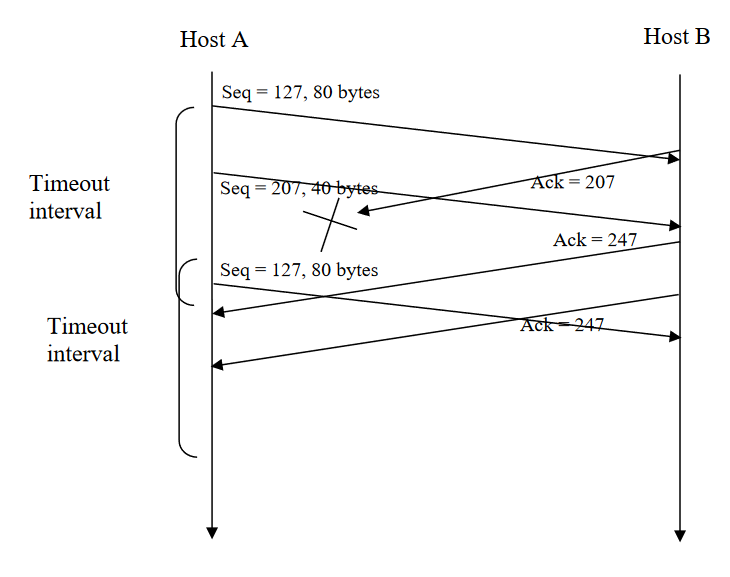
\includegraphics[width=0.8\linewidth]{1.png}
              \caption{}\label{A}
            \end{figure}
            \newpage
    \end{enumerate}

    \section{P28. El host A y B est\'an conectados directamente con un enlace de 100 Mbps. Hay una conexi\'on TCP entre los dos hosts, y Host A est\'a enviando a Host B un archivo enorme sobre esta conexi\'on. Host A puede enviar sus datos de la aplicaci\'on a su z\'ocalo TCP a una velocidad de hasta 120 Mbps, pero Host B puede leer de su b\'ufer de recepci\'on TCP a una velocidad m\'axima de 50 Mbps. Describir el efecto del control de flujo TCP.}
    Dado que la capacidad del enlace es de solo 100 Mbps, la velocidad de env\'io del host A puede ser como m\'aximo de 100 Mbps. A\'un as\'i, el host A env\'ia datos al b\'ufer de recepci\'on más r\'apido de lo que el host B puede eliminar datos del b\'ufer. El b\'ufer de recepci\'on se llena a una velocidad de aproximadamente 40 Mbps. Cuando el b\'ufer est\'a lleno, el Host B le indica al Host A que deje de enviar datos configurando RcvWindow $=$ 0. \\
    Host A entonces deja de enviar hasta que recibe un segmento TCP con RcvWindow $>$ 0. Por lo tanto, el host A detendr\'a repetidamente un env\'io d start en funci\'on de los valores RcvWindow que recibe del Host B. En promedio, la tasa a largo plazo a la que el Host A env\'ia datos al Host B como parte de esta conexi\'on no es m\'as de 60 Mbps.

    \section{P29. Las cookies SYN se discutieron en la secci\'on 3.5.6 .}
    \textbf{\begin{enumerate}
              \item ?`Por qu\'e es necesario que el servidor utilice un n\'umero de secuencia inicial especial en la SYNACK?
              \item Supongamos que un atacante sabe que un host de destino utiliza cookies SYN. ?`Puede el atacante crear conexiones semiabiertas o totalmente abiertas simplemente enviando un paquete ACK al destino? ?`Por qu\'e o por qu\'e no?
              \item Supongamos que un atacante recoge una gran cantidad de n\'umeros de secuencia iniciales enviados por el servidor. ?`Puede el atacante hacer que el servidor cree muchas conexiones completamente abiertas enviando ACKs con esos n\'umeros de secuencia iniciales? ?`Por qu\'e?
            \end{enumerate}}

    \textbf{Respuesta:}
    \begin{enumerate}
      \item El servidor utiliza un n\'umero de secuencia inicial especial (que se obtiene a partir del hash de las IPs y puertos de origen y destino) para defenderse del ataque SYN FLOOD.
      \item No, el atacante no puede crear conexiones semiabiertas o totalmente abiertas simplemente enviando paquetes ACK al destino. Las conexiones semiabiertas no son posibles ya que un servidor que utiliza cookies SYN no mantiene variables de conexi\'on y buffers para ninguna conexi\'on antes de que se establezcan conexiones completas. Para establecer conexiones completamente abiertas, un atacante debe conocer el n\'umero de secuencia inicial especial correspondiente a la direcci\'on IP de origen (falsificada) del atacante. Este n\'umero de secuencia requiere el n\'umero "secreto" que cada servidor utiliza. Dado que el atacante no conoce este n\'umero secreto, no puede adivinar el n\'umero de la secuencia inicial.
      \item No, el sever simplemente puede a\~{n}adir una marca de tiempo al calcular esos n\'umeros de secuencia iniciales y elegir un valor de tiempo para vivir para esos n\'umeros de secuencia, y descartar los n\'umeros de secuencia iniciales expirados incluso si el atacante los repite.
    \end{enumerate}

    \section{P33. En la Secci\'on 3.5.3, discutimos la estimaci\'on de RTT de TCP. ?`Por qu\'e crees que TCP evita medir el SampleRTT para segmentos retransmitidos?}
    Veamos lo que podr\'ia estar mal si TCP mide SampleRTT para un segmento retransmitido. Supongamos que la fuente env\'ia el paquete P1, el temporizador para P1 expira, y la fuente entonces env\'ia P2, una nueva copia del mismo paquete. Supongamos adem\'as que la fuente mide SampleRTT para P2 (el paquete retransmitido). Finalmente supongamos que poco despu\'es de transmitir P2 llega un acuse de recibo para P1. La fuente tomar\'a err\'oneamente este reconocimiento como un reconocimiento para P2 y calcular\'a un valor incorrecto de SampleRTT.\\
    Veamos lo que podr\'ia estar mal si TCP mide SampleRTT para un segmento retransmitido. Supongamos que la fuente env\'ia el paquete P1, el temporizador para P1 expira, y la fuente entonces env\'ia P2, una nueva copia del mismo paquete. Supongamos adem\'as que la fuente mide SampleRTT para P2 (el paquete retransmitido). Finalmente supongamos que poco despu\'es de transmitir P2 llega un acuse de recibo para P1. La fuente tomar\'a err\'oneamente este reconocimiento como un reconocimiento para P2 y calcular\'a un valor incorrecto de SampleRTT .

    \section{P40. Considere la Figura 3.58 . Asumiendo que TCP Reno es el protocolo que experimenta el comportamiento mostrado arriba, responda las siguientes preguntas. En todos los casos, debe proporcionar una breve discusi\'on que justifique su respuesta.}
    \textbf{\begin{enumerate}
              \item Identifique los intervalos de tiempo en los que el inicio lento de TCP est\'a funcionando.
              \item Identifique los intervalos de tiempo en los que funciona la prevenci\'on de congesti\'on de TCP.
              \item Despu\'es de la 16a ronda de transmisi\'on, ?`se detecta la p\'erdida de segmento mediante un ACK triple duplicado o por un tiempo de espera?
              \item Despu\'es de la $22$ ronda de transmisi\'on, ?`se detecta la p\'erdida de segmento por un triple duplicado ACK o por un tiempo de espera?
              \begin{figure}
                \centering
                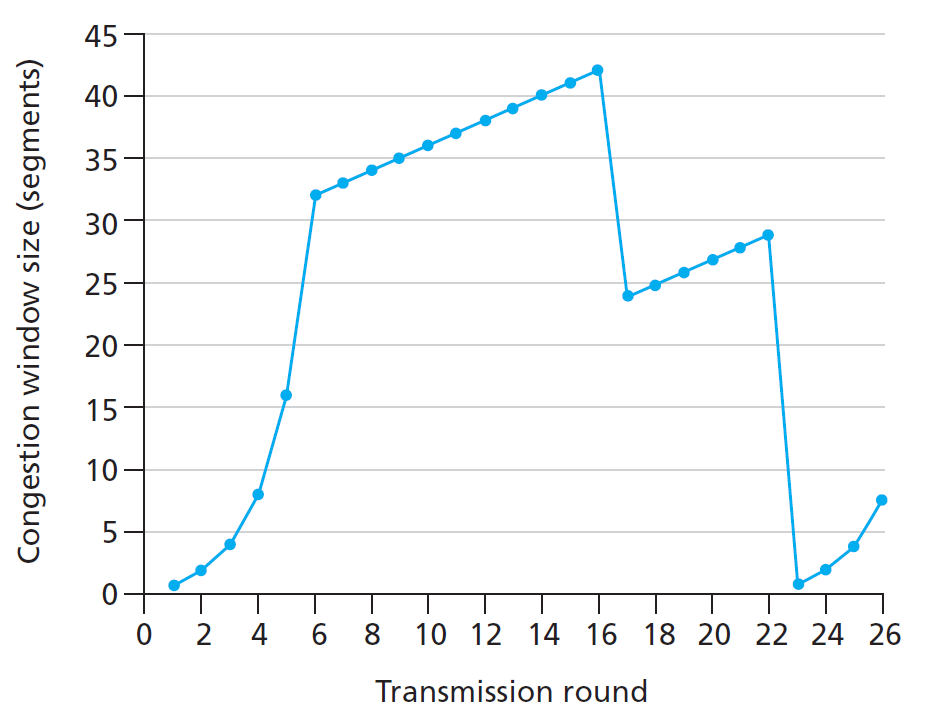
\includegraphics[width=0.5\linewidth]{2.png}
                \caption{TCP window size as a function of time}\label{2}
              \end{figure}
              \item ?`Cu\'al es el valor inicial de ssthresh en la primera ronda de transmisi\'on?
              \item ?`Cu\'al es el valor de ssthresh en la $18$ ronda de transmisi\'on?
              \item ?`Cu\'al es el valor de ssthresh en la $24$ ronda de transmisi\'on?
              \item ?`Durante qu\'e ronda de transmisi\'on se envía el segmento 70?
              \item Suponiendo que se detecta la p\'erdida de un paquete despu\'es de la $26a$ ronda mediante la recepci\'on de un triple ACK duplicado, ?`cu\'ales ser\'an los valores del tama\~{n}o de la ventana de congesti\'on y de ssthresh?
              \item Suponga que se usa TCP Tahoe (en lugar de TCP Reno), y asuma que los ACK duplicados triples se reciben en la $16$ ronda. ?`Cu\'ales son los ssthresh y el tama\~{n}o de la ventana de congesti\'on en la $19$ ronda?
              \item De nuevo supongamos que se utiliza TCP Tahoe, y hay un evento de tiempo de espera en la ronda 22. ?`Cu\'antos paquetes se han enviado desde la ronda 17 hasta la ronda 22?
            \end{enumerate}}

    \textbf{Respuesta:}
    \begin{enumerate}
      \item TCP slowstart est\'a operando en los intervalos [1,6] y [23,26]
      \item TCP congestion avoidance est\'a operando en los intervalos [6,16] y [17,22]
      \item Despu\'es del 16 ronda de transmisi\'on, la p\'erdida de paquetes se reconoce mediante un triple ACK duplicado. Si hubiera un tiempo de espera, el tama\~{n}o de la ventana de congesti\'on se habr\'ia reducido a 1.
      \item Despu\'es de la 22 ronda de transmisi\'on, la p\'erdida de segmento se detecta debido al tiempo de espera, y por lo tanto el tama\~{n}o de la ventana de congesti\'on se establece en 1.
      \item El umbral es inicialmente 32, ya que es en este tama\~{n}o de ventana donde se detiene el slow start y comienza la evitaci\'on de la congesti\'on.
      \item El umbral se establece en la mitad del valor de la ventana de congesti\'on cuando se detecta la p\'erdida de paquetes. Cuando se detecta una p\'erdida durante la ronda 16 de transmisi\'on, el tama\~{n}o de las ventanas de congesti\'on es 42. Por tanto, el umbral es 21 durante la ronda 18 de transmisi\'on.
      \item El umbral se establece a la mitad del valor de la ventana de congesti\'on cuando se detecta la p\'erdida de paquetes. Cuando la p\'erdida se detecta durante la ronda de transmisi\'on 22, el tama\~{n}o de las ventanas de congesti\'on es 29. Por lo tanto el umbral es 14 (tomando el piso inferior de 14.5) durante la 24 ronda de transmisi\'on.
      \item Durante la primera ronda de transmisi\'on, se env\'ia el paquete 1; el paquete 2-3 se env\'ia en la segunda ronda de transmisi\'on; los paquetes 4-7 se env\'ian en la tercera ronda de transmisi\'on; los paquetes 8-15 se env\'ian en la cuarta ronda de transmisi\'on; los paquetes 16-31 se env\'ian en la quinta ronda de transmisi\'on; los paquetes 32-63 se env\'ian en la 6 ronda de transmisi\'on; los paquetes 64-96 se env\'ian en la 7 ronda de transmisi\'on. As\'i, el paquete 70 se env\'ia en la s\'eptima ronda de transmisi\'on.
      \item El umbral se fijar\'a a la mitad del valor actual de la ventana de congesti\'on (8) cuando se produzca la p\'erdida y la ventana de congesti\'on se fijar\'a al nuevo valor de umbral + 3 SMS . As\'i, los nuevos valores del umbral y de la ventana ser\'an 4 y 7 respectivamente.
      \item El umbral es 21 y el tama\~{n}o de la ventana de congesti\'on es 1.
      \item Ronda 17, 1 paquete;\\
            Ronda 18, 2 paquetes; \\
            Ronda 19, 4 paquetes;\\
            Ronda 20, 8 paquetes; \\
            Ronda 21, 16 paquetes; \\
            Ronda 22, 21 paquetes. \\
            Entonces, el n\'umero total es 52.
    \end{enumerate}




\end{document} 